\documentclass{article}

\usepackage[colorlinks=true]{hyperref}
\usepackage{amsmath}
\usepackage{graphicx}
\usepackage{float}
\usepackage{geometry} 
\usepackage{hyperref}
\usepackage{algorithm}
\usepackage{graphicx}
\usepackage{algpseudocode}

\begin{document}

\title{Efficient State Enumeration in a Torus Grid World: Algorithms and Analysis}
\author{Vasil Dakov}
\date{}
\maketitle

\begin{abstract}
    We address the problem of state enumeration in a torus grid world with unknown dimensions and starting state. The goal is to ensure that every state is visited while maintaining an algorithmic complexity of $O(35S)$, where $S = w \cdot h$ is the area of the torus. We present and analyze a baseline spiral algorithm and an improved approach leveraging irrational slopes to ensure termination and efficiency. Theoretical guarantees and empirical observations are provided to validate the proposed solutions.
\end{abstract}

\section{Problem Overview}
We define the problem as a search task in a $w \times h$ torus grid world. The
state space is defined as:
\[
    \mathcal{S} = \{(i, j) \mid \forall i, j: 0 \leq i < w, 0 \leq j < h\}.
\]

The agent has no prior knowledge of the world's dimensions or its initial
state. The action space is given by:
\[
    \mathcal{A} = \{(i, (j + 1) \mod h), (i, (j - 1) \mod h), ((i + 1) \mod w, j), ((i - 1) \mod w, j)\}.
\]

The objective is to reach a goal state, which can be any state in
$\mathcal{S}$. Without loss of generality, the problem can be reformulated as
visiting all states in $\mathcal{S}$, leveraging the torus's wrap-around
property.

Several mathematical properties of our environment and solution must be defined
to proceed.

We can reformulate the problem as visiting all possible spaces on the torus.
This is due to the fact that we have no knowledge of the environment and the
goal can be on any single state. This reformulation gives the freedom to start
from an arbitrary location- starting location is irrelevant for the torus'
enumeration due to its wrap-around.

\section{Solution}
To be sure all spots on the torus are visited, we must ensure our algorithm
never enters a periodic cycle prior to enumerating the whole torus. Otherwise,
that would leave edge cases with some unenumberated state(s). For example, a
simple diagonal policy ($right \to down \to right \to down$) would enter a
cycle on $4 \times 4$ grid.

\subsection*{Baseline solution}
The simplest solution with a guarantee of enumerating all states is a spiral
outward. It only requires knowledge of the initial state. In all cases, it
would steadily grow toward unvisited states, assuring eventually all states are
visited (and consequently the goal state). Pseudocode provided in
\autoref{alg:spiral} along with a visualization in
\autoref{fig:visualization-of-spiral-algorithm}. Unfortunately its runtime
comlexity is quadratic with respect to the larger side of the grid: $\mathbf
    O(\max(w, h)^2)$, as the spiral will always enumerate a square with sides equal
to the larger side. In many cases this violates our $\mathbf O(35\cdot S)$
restriction. For example, for $w=1, h = 10^6$, the algorithm would do $10^{12}$
steps or $S \cdot 10^6 S$

\begin{figure}[H]
    \centering
    \begin{minipage}{0.5\textwidth}
        \begin{algorithm}[H]
            \caption{Spiral Movement Policy}\label{alg:spiral}
            \begin{algorithmic}[1]
                \Require Grid dimensions, current position $(nx, ny)$, and global variables: \texttt{counter}, \texttt{step\_size}, \texttt{direction}.
                \Ensure Next position $(nx, ny)$.
                \State Extract $nx, ny$ from the current position.
                \If{\texttt{direction} = 0} \Comment{Move right}
                \State $nx \gets (nx + 1) \bmod \texttt{width}$
                \ElsIf{\texttt{direction} = 1} \Comment{Move down}
                \State $ny \gets (ny - 1) \bmod \texttt{height}$
                \ElsIf{\texttt{direction} = 2} \Comment{Move left}
                \State $nx \gets (nx - 1) \bmod \texttt{width}$
                \ElsIf{\texttt{direction} = 3} \Comment{Move up}
                \State $ny \gets (ny + 1) \bmod \texttt{height}$
                \EndIf
                \State \texttt{counter} $\gets$ \texttt{counter} $+ 1$
                \If{\texttt{counter} = \texttt{step\_size}}
                \State \texttt{counter} $\gets 0$
                \State \texttt{direction} $\gets (\texttt{direction} + 1) \bmod 4$
                \If{\texttt{direction} is even}
                \Comment{Increase step size after right/down or left/up}
                \State \texttt{step\_size} $\gets \texttt{step\_size} + 1$
                \EndIf
                \EndIf
                \State \Return $(nx, ny)$
            \end{algorithmic}
        \end{algorithm}

    \end{minipage}
    \hfill
    \begin{minipage}{0.45\textwidth}
        \centering
        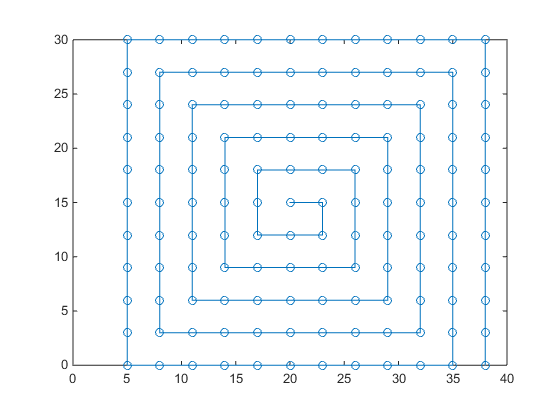
\includegraphics[width=\linewidth]{grid_spiral.png}
        \caption{How the spiral algorithm looks like. It is visible how it grows outward and would eventually cover the entire grid. Image credit: \url{https://stackoverflow.com/questions/29466058/spiral-loop-on-a-matrix-from-a-point}}
        \label{fig:visualization-of-spiral-algorithm}
    \end{minipage}
\end{figure}

\subsection*{Improved Solution}

My solution greatly improves on edge cases like the one in the baseline
solution, while staying linear. It is a diagonal algorithm, iterating in the
$x-$ and $y-$ axes by taking steps along an irrational slope with steps sizes
$\Delta x = (\sqrt 5 - 1)/2$ and $\Delta y = 1$. It guarantees that it
enumerates the grid due to the mathematical properties of irrational numbers,
low-discrepancy sequences and the torus itself. Pseudocode provided in
\autoref{alg:diagonal}.

\subsection*{Why this solution works}
Here is a brief overview of the properties that guarantee the effectiveness and
termination of my solution.

\textbf{Guarantee of termination:} We can use the irrational winding of the torus theorem to guarantee that all spots on the torus are covered. It states that, for an
$n$-dimensional torus, a line with an irrational slope is dense on the torus (or covers all points on it when traced for long enough)\cite{irrational-torus}. Conversely, a rational slope forms a closed line.

Our environment torus is slightly different as it is discrete. As such, we are
doing an approximation of the irrational winding of the torus, by iterating in
both directions and rounding up to the nearest index. The slope is assured to
be irrational, as $\Delta x = (\sqrt 5 - 1)/2$ is irrational - $\Delta y$ does
not need to be irrational to satisfy this and empirical experiements showed $
    \Delta y=1$ provides faster termination. Intuitively, we have an irrational
slope, and irrational numbers have the property of being aperiodic, meaning
with enough iterations a solution will always be found.

\textbf{Efficiency:}

The algorithm empirically has shown to perform much better than the baseline
solution, and also has the theoretical properties to back it up. Iterating
irrational steps additively gives what is called a \textit{low-discrepancy
    sequence} \cite{low-discrepancy-seq}. It is an approximation of how well all
sizes of that subsequence fall into an equidistributed (uniformly distributed)
sequence. In other words, it is a measure of the dissimilarity with a uniform
distribution. For irrational numbers, and large sequences, it is proven that
the discrepancy D tends to $\frac{1}{N}$ where $N$ is the number of elements in
the sequence. For our problem, this is limited to $\frac{1}{35\cdot S}$. If we
assume to have achieved this low discrepancy, we can restate the problem as a
covering of the unit circle via a uniform distribution. This is equivalent to
the coupon collector's problem from probability theory \cite{coupon-collector}.
It gives us an upper bound of the number of steps we may need to take to
enumerate the unit circle.

This upper bound is ${E} (T)=S\cdot H_{S}=S\log S+\gamma S+{\frac
    {1}{2}}+O(1/S)$ where $T$ is the number of steps expected to cover the square,
$S$ is the area of the grid, $H_S$ is the $S$th harmonic number and $\gamma
    \approx 0.577215...$ or the Euler-Mascheroni constant \cite{coupon-collector}.

Naturally, there is clumsiness here due to our assumptions and the the discrete
nature of our torus, and for how large the $N$ needs to be to ensure low
discrepancy. Empirically, however, the approximation seems to be good enough,
results ranged between $[1 \cdot S, 18\cdot S]$, well in the limits. . Some
edge cases might be possible, however, violating the $O(35\cdot S) $
constraint. This is also dependent on the step-size, where the golden ration I
used has better theoretical properties.

\begin{figure}[H]
    \centering
    \begin{minipage}{0.5\textwidth}
        \begin{algorithm}[H]
            \caption{Irrational Movement Policy}\label{alg:diagonal}
            \begin{algorithmic}[1]
                \Require Grid dimensions, current position $(nx, ny)$, goal position, and global variable: \texttt{counter}.
                \Ensure Next position $(nx, ny)$.
                \State Extract $nx, ny$ from the current position.
                \State $\Delta_x \gets (\sqrt{5} - 1) / 2$ \Comment{Golden ratio adjustment}
                \State $\Delta_y \gets 1$
                \If{\texttt{counter} = 0} \Comment{Adjust $x$ coordinate}
                \State $nx \gets (nx + \Delta_x) \bmod \texttt{width}$
                \ElsIf{\texttt{counter} = 1} \Comment{Adjust $y$ coordinate}
                \State $ny \gets (ny + \Delta_y) \bmod \texttt{height}$
                \EndIf
                \State \texttt{counter} $\gets (\texttt{counter} + 1) \bmod 2$
                \State \Return $(nx, ny)$
            \end{algorithmic}
        \end{algorithm}
    \end{minipage}
    \hfill
    \begin{minipage}{0.45\textwidth}
        \centering
        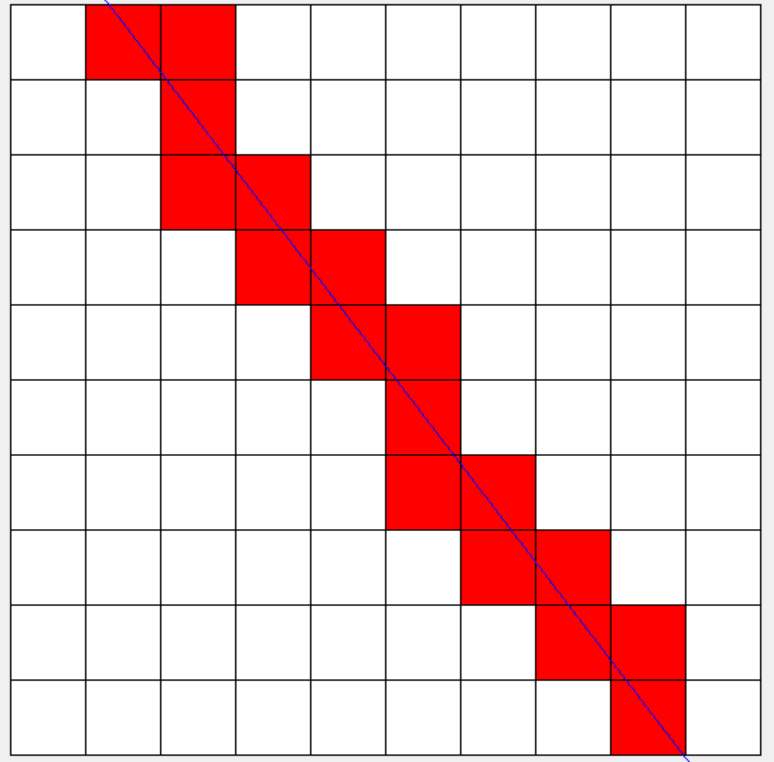
\includegraphics[width=\linewidth]{grid_irrational.png}
        \caption{Approximate vissualization of the irrational grid policy. Image credit: \url{https://i.sstatic.net/MIt2B.png}}
        \label{fig:visualization-of-diagonal-algorithm}
    \end{minipage}
\end{figure}

Various grid sizes were tested, symmetric, non symmetric, heavily skewed, and
such to ensure all properties were tested. Some examples are: (3, 3), (4, 5),
(9, 9), (100, 100), (1000, 1000), (1, 10), (1, 1000), (1000, 1), (1, 1000000),
(500, 500), (250, 400), (50, 50), (25, 40), (2, 5000).

\section{Alternatives considered}

Creating heuristics was an alternative considered for this task. Most
predominantly, Euclidean distance was tested modularly, to ensure admissibility
and consistency on the sequence created. As expected, it performs optimally and
finds the shortest part of the goal each time. In general, all heuristics seemed to give 
away some spatial information. This was deemed "cheating" and
violating the problem conditions, however, as we were giving the agent
information on the location of the goal.

\bibliographystyle{plain}
\bibliography{src}

\end{document}

